\lab{Algorithm}{Image Segmentation with Minimal Spanning Trees}{Image Segmentation with Minimal Spanning Trees}
\label{Ch:MSTImgSeg}

\objective{This section teaches about how to use minimum spanning trees to segment an image.}

\section*{Image Segmentation}

%Lab \ref{MSTImgSeg}

One application of Minimal Spanning Trees (MSTs) is image segmentation.
Kruskal's algorithm is especially good at this.
Let $k$ be the number of divisions that is wanted and $n$ be the number of nodes.
Kruskal's algorithm is performed until $n-k$ edges are added.

There are many different ways to turn an image into a graph and weight the edges.
A simple, yet effective, version is to make every pixel a node and the edges are the difference in intensities in the four cardinal directions. 

This means that there are less than $4n$ edges.
Other image segmentation algorithms have to use $n^2$ space.
This gives the MST algorithm a critical advantage over other image segmentation algorithms. 

\begin{problem}
Write a function that takes a black and white image as input and outputs a list of the edges and a list of nodes.
Store the edges using the form \li{(node,node,weight)}.
\end{problem}

The provided Kruskal's algorithm takes as inputs the list of nodes, the list of edges and the number of divisions desired.
The number of divisions often has to be higher than the actual number that is needed because sometimes one or two pixels form a division because the difference between them and the pixels around them is so great.
You will have to adjust the number of divisions until the desired result is found.

\begin{problem}
Perform the image segmentation algorithm on the image, then graph the original image and the three largest divisions.
(Use the Counter class from collections to find the number of pixels in each division.) 
\end{problem}

\vfill
\begin{figure}[ht]
\begin{minipage}[b]{0.47\linewidth}
\centering

\includegraphics[width=\textwidth]{MSTseg1.jpg}
\end{minipage}
\hspace{0.5cm}
\begin{minipage}[b]{0.47\linewidth}
\centering
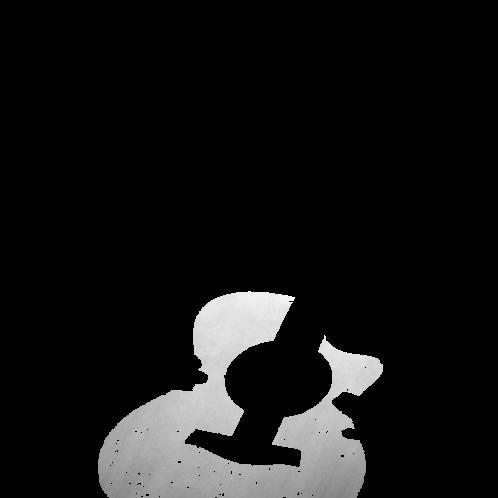
\includegraphics[width=\textwidth]{MSTseg2.jpg}
\end{minipage}
\begin{minipage}[b]{0.47\linewidth}
\centering

\includegraphics[width=\textwidth]{MSTseg3.jpg}
\end{minipage}
\hspace{0.5cm}
\begin{minipage}[b]{0.47\linewidth}
\centering
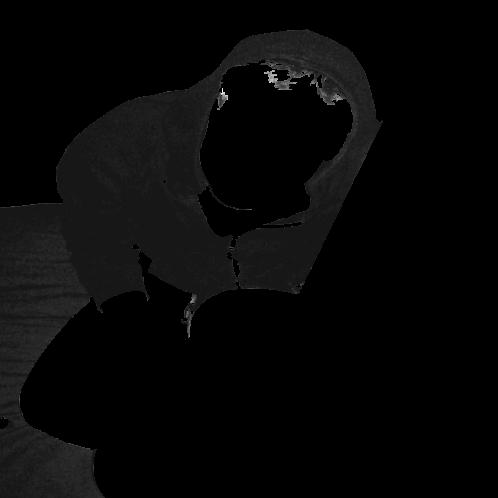
\includegraphics[width=\textwidth]{MSTseg4.jpg}
\end{minipage}
\caption{The original image is in the top left hand corner. The three larges segments are shown in the other corners. The original image was 498x498 and 50000 divisions were used. TODO get permission to use this picture}
\end{figure}
\vfill

\begin{problem}
Make a division of the image a different color.
\end{problem}

This algorithm can also be extended to 3D images.
One way to do this is to make each pixel a node and have the edges run in the eight cardinal directions, i.e. the pixel directly above it, the pixel below it, etc.

This algorithm can also be used to segment other data such as connections on Facebook. 
